通过使用noexcept关键字的示例来开始这个主题。\par

\hspace*{\fill} \par %插入空行
\textbf{7.1.1 无noexcept的移动构造函数}

下面的类,引入了带有string成员的类型,并实现了复制和移动构造函数:\par

{\color{red}{basics/person.hpp}}\par

\begin{lstlisting}[caption={}]
#include <string>
#include <iostream>

class Person {
	private:
	std::string name;
	public:
	Person(const char* n)
	: name{n} {
	}

	std::string getName() const {
		return name;
	}

	// print out when we copy or move:
	Person(const Person& p)
	: name{p.name} {
		std::cout << "COPY " << name << '\n';
	}
	Person(Person&& p)
	: name{std::move(p.name)} {
		std::cout << "MOVE " << name << '\n';
	}
	...
};
\end{lstlisting}

现在创建并初始化一个\textit{Person}的vector,并插入一个\textit{Person}对象:\par

{\color{red}{basics/person.cpp}}\par

\begin{lstlisting}[caption={}]
#include "person.hpp"
#include <iostream>
#include <vector>

int main()
{
	std::vector<Person> coll{"Wolfgang Amadeus Mozart",
		"Johann Sebastian Bach",
		"Ludwig van Beethoven"};
	std::cout << "capacity: " << coll.capacity() << '\n';
	coll.push_back("Pjotr Iljitsch Tschaikowski");
}
\end{lstlisting}

程序输出如下:\par

\begin{tcolorbox}[colback=white,colframe=black]
COPY Wolfgang Amadeus Mozart \\
COPY Johann Sebastian Bach \\
COPY Ludwig van Beethoven \\
capacity: 3 \\
MOVE Pjotr Iljitsch Tschaikowski \\
COPY Wolfgang Amadeus Mozart \\
COPY Johann Sebastian Bach \\
COPY Ludwig van Beethoven
\end{tcolorbox}

首先,将初始值复制到vector中(容器的std::initializer\_list<>构造函数按值接受传递的参数)。因此,vector通常为三个元素分配内存:\par

\begin{center}
	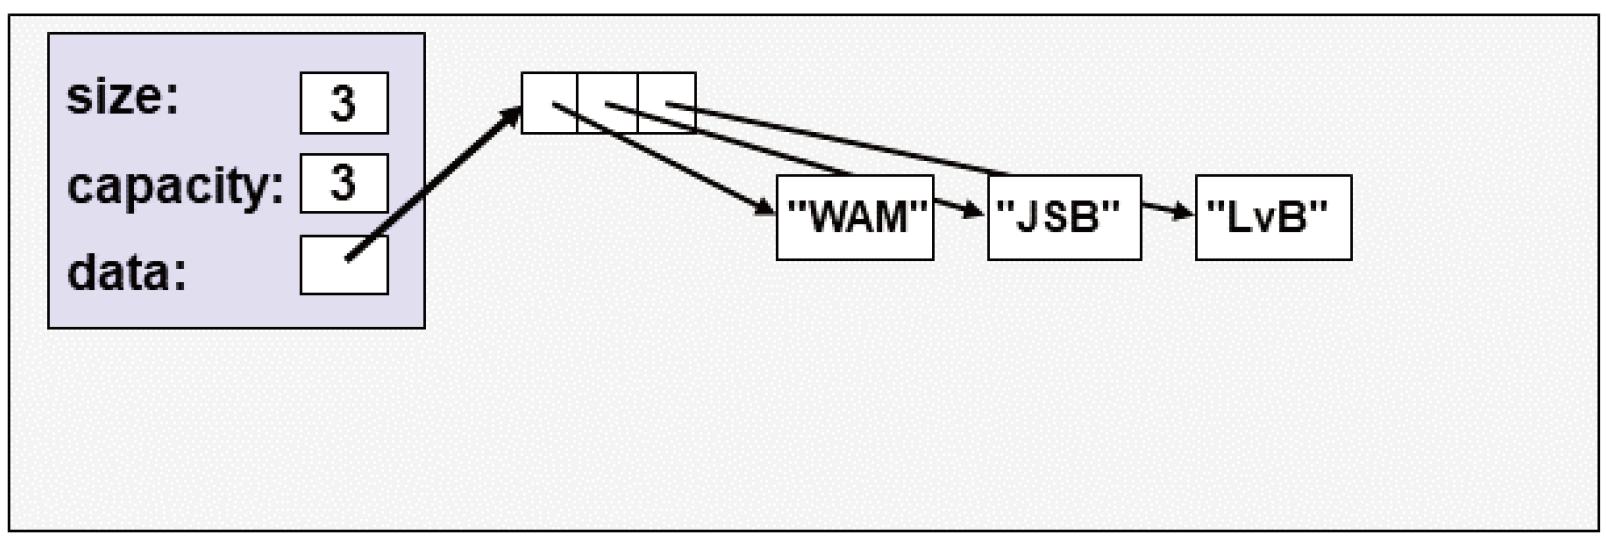
\includegraphics[width=1.0\textwidth]{content/1/chapter7/images/1}
\end{center}

接下来会发生什么:用push\_back()插入第四个元素,结果如下:\par

\begin{itemize}
	\item vector在内部需要更多内存,所以会分配新的内存(比如,6个元素),移动第4个字符串(创建一个临时的\textit{Person}并使用\textit{push\_back()}方法将其移动到vector中),但也会将现有的元素复制到新内存中:\par
	\begin{center}
		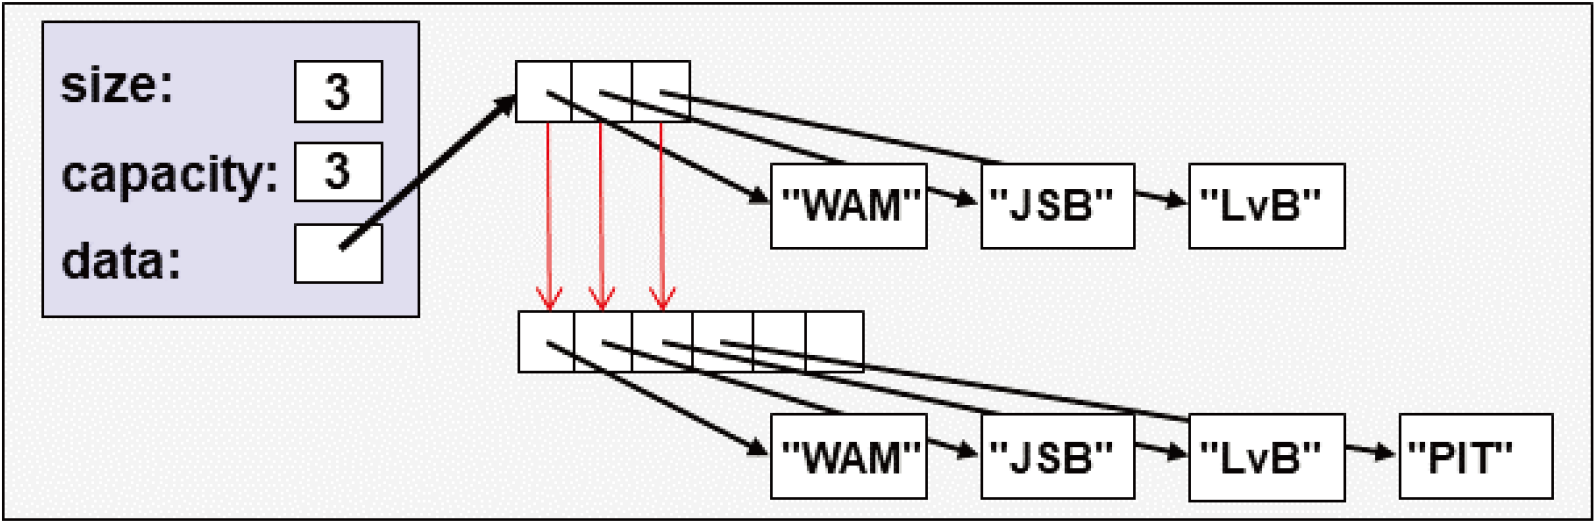
\includegraphics[width=1.0\textwidth]{content/1/chapter7/images/2}
	\end{center}
	\item 这个操作结束时,vector销毁旧的元素,释放这些元素的旧内存,并更新成员:\par
	\begin{center}
		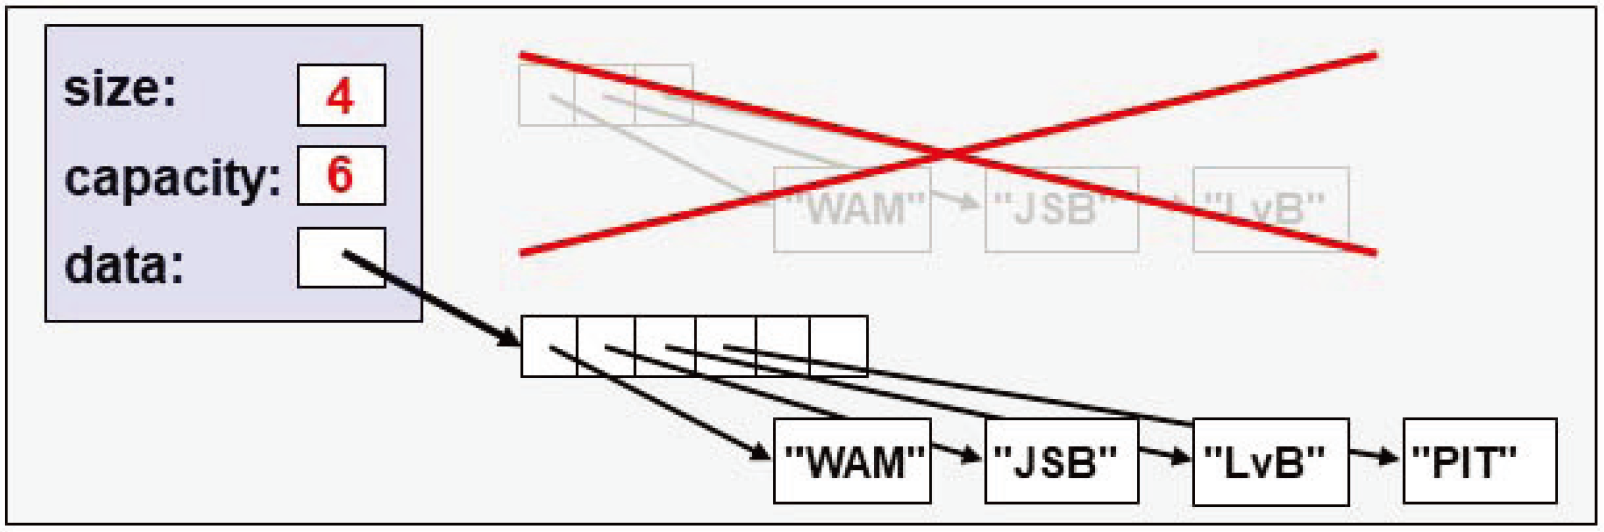
\includegraphics[width=1.0\textwidth]{content/1/chapter7/images/3}
	\end{center}
\end{itemize}

问题是,为什么vector不使用移动构造函数,将元素从旧内存移动到新内存呢?\par

\hspace*{\fill} \par %插入空行
\textbf{强异常安全保证}

vector的重新分配不使用移动语义的原因是,\textit{push\_back()}提供了强异常处理保证:在vector的重新分配过程中抛出异常时,C++标准库保证将vector回退到之前的状态。也就是说,\textit{push\_back()}提供了一种保证:要么成功,要么无效。\par

C++标准能够在C++98和C++03中提供这种保证,因为C++只能复制元素。如果在复制元素时出现错误,源对象仍然可用。处理异常的内部代码只需销毁创建的副本,并释放新的内存,使vector返回到之前的状态(C++标准库要求析构函数不抛出异常;否则,无法回退)。\par

重新分配是使用移动语义的最优位置,因为只是元素从一个位置移动到另一个位置。因此,C++11希望在这里使用移动语义。但是,如果在重新分配期间抛出异常,就无法回退了。新内存中的元素已经窃取了旧内存中元素的值。因此,只是销毁新的元素还不够,还得把他们移回去。但怎么知道把移回去的时候就不会失败呢?\par

你可能会说一个移动构造函数永远不抛出异常。这可能是正确的字符串(因为我们只是移动值和指针),而是需要对象在一个有效的状态,这种状态可能需要额外的内存,所以当额外内存有问题时会丢弃状态信息(例如,基于节点的容器Visual C++实现方式)。\par

我们也不能放弃,因为程序可能已经使用这个特性来避免创建向量的备份,而丢失数据可能是(安全)关键的。不再支持push\_back()对于使用C++11来说将是个噩梦。\par

最后,只有当元素类型的移动构造函数保证不抛出异常时,才在重新分配时使用移动语义。\par

\hspace*{\fill} \par %插入空行
\textbf{7.1.2 使用noexcept的移动构造函数}

因此,保证\textit{Person}类的移动构造函数永远不会抛出异常时,示例程序就改变了行为:\par

{\color{red}{basics/personmove.hpp}}\par

\begin{lstlisting}[caption={}]
#include <string>
#include <iostream>

class Person {
	private:
	std::string name;
	public:
	Person(const char* n)
	: name{n} {
	}
	std::string getName() const {
		return name;
	}

	// print out when we copy or move:
	Person(const Person& p)
	: name{p.name} {
		std::cout << "COPY " << name << '\n';
	}
	Person(Person&& p) noexcept // guarantee not to throw
	: name{std::move(p.name)} {
		std::cout << "MOVE " << name << '\n';
	}
	...
};
\end{lstlisting}

如果像以前一样使用\textit{Persons}:\par

{\color{red}{basics/personmove.cpp}}\par

\begin{lstlisting}[caption={}]
#include "personmove.hpp"
#include <iostream>
#include <vector>

int main()
{
	std::vector<Person> coll{"Wolfgang Amadeus Mozart",
		"Johann Sebastian Bach",
		"Ludwig van Beethoven"};
	std::cout << "capacity: " << coll.capacity() << '\n';
	coll.push_back("Pjotr Iljitsch Tschaikowski");
}
\end{lstlisting}

可得到以下输出:\par

\begin{tcolorbox}[colback=white,colframe=black]
COPY Wolfgang Amadeus Mozart \\ 
COPY Johann Sebastian Bach \\
COPY Ludwig van Beethoven \\
capacity: 3 \\
MOVE Pjotr Iljitsch Tschaikowski \\
MOVE Wolfgang Amadeus Mozart \\
MOVE Johann Sebastian Bach \\
MOVE Ludwig van Beethoven
\end{tcolorbox}

同样,首先将初始值复制到vector中\par

\begin{center}
	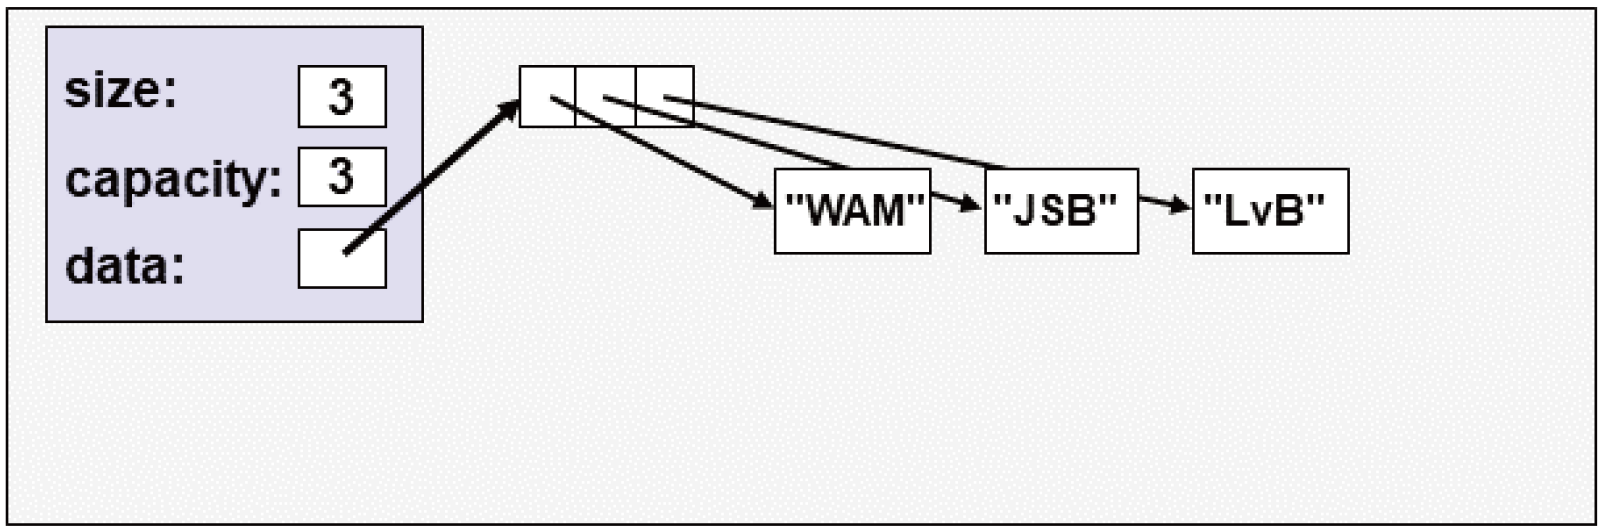
\includegraphics[width=1.0\textwidth]{content/1/chapter7/images/4}
\end{center}

然而,随着输出的最后三行可视化,vector现在使用移动构造函数将元素移动到新的重新分配的内存中:\par

\begin{center}
	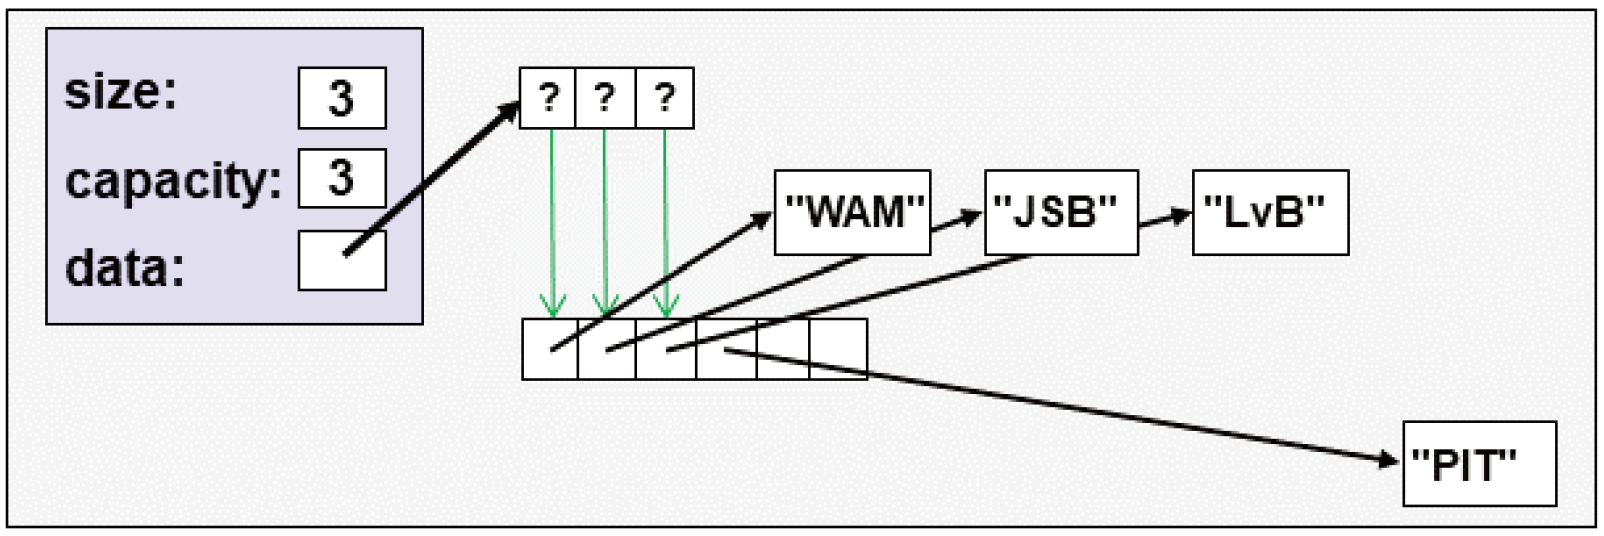
\includegraphics[width=1.0\textwidth]{content/1/chapter7/images/5}
\end{center}

最后,vector只需要释放旧内存并更新其成员:\par

\begin{center}
	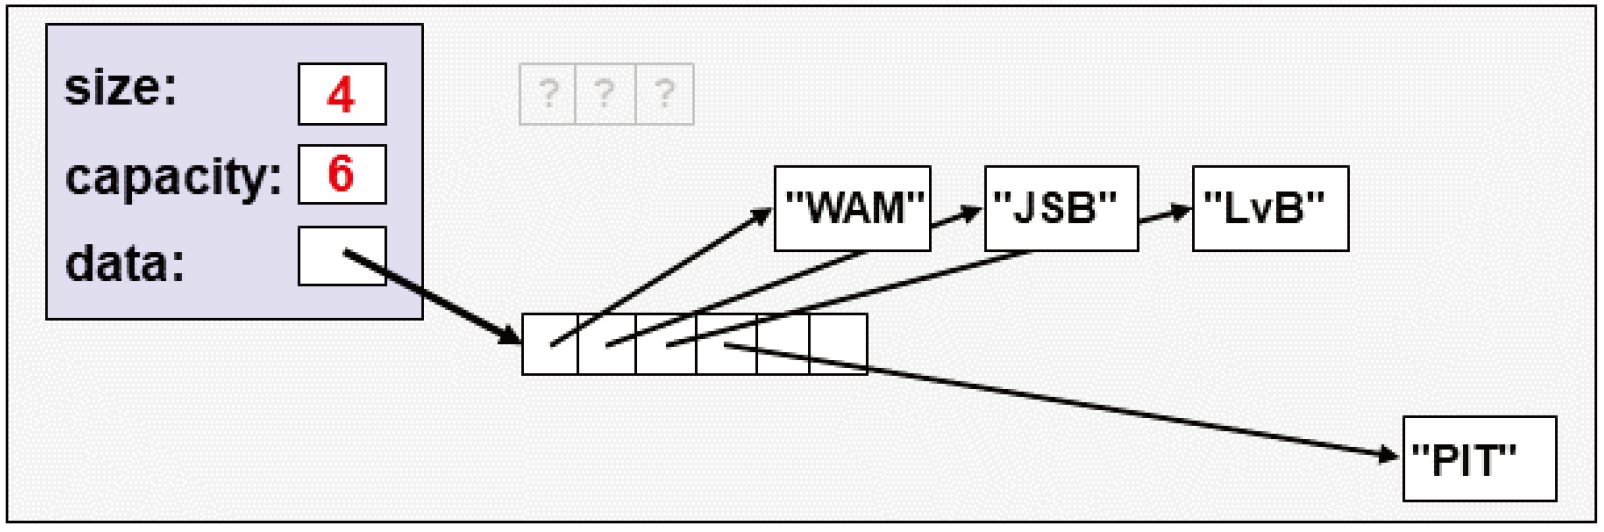
\includegraphics[width=1.0\textwidth]{content/1/chapter7/images/6}
\end{center}

\hspace*{\fill} \par %插入空行
\textbf{具有条件的noexcept声明}

然而,是否可以将移动构造函数标记为noexcept?移动\textit{name}(一个std::string),并向标准输出流写入一些内容。如果在那里抛出异常,就违反了无异常的保证。这种情况下,程序在运行时将调用std::terminate(),后者通常调用std::abort()来发出程序异常结束的信号(通常会出现core dump)。\par

因此,如果string成员和输出操作不抛出异常,则应该保证不抛出异常。引入noexcept关键字是用来指定不抛出的条件保证。({\color{red}{basics/personcond.hpp}}是一个完整的例子):\par

\begin{lstlisting}[caption={}]
class Person {
	private:
		std::string name;
	public:
		...
		Person(Person&& p)
		noexcept(std::is_nothrow_move_constructible_v<std::string>
		&& noexcept(std::cout << name))
		: name{std::move(p.name)} {
			std::cout << "MOVE " << name << '\n';
		}
		...
\end{lstlisting}

使用noexcept(…),保证括号内的编译时表达式为真时不会抛出异常。这种情况下,需要两样东西来保证:\par

\begin{itemize}
	\item 对于std::is\_nothrow\_move\_constructible\_v<std::string>(在C++20之前,必须使用std::is\_nothrow\_move\_constructible<std::string>::value),使用标准类型特征(type)来告诉std::string的移动构造函数是否保证不抛出异常。
	\item 对于noexcept(std::cout << name),对名称的输出表达式是否保证不抛出异常。这里,使用noexcept作为操作符,说明是否所有执行传递的表达式都保证不会抛出异常。
\end{itemize}

通过此声明,重新分配将再次使用复制构造函数。字符串的移动构造函数不保证抛出异常,但输出操作符不保证抛出异常。然而,移动构造函数通常不输出任何内容。因此,通常当成员不抛出异常时,可以为整个移动构造函数提供不抛出异常的保证。\par

好消息是,如果没有自己实现移动构造函数,编译器将为你提供noexcept保证。对于所有成员都保证不抛出移动构造函数的类,生成的或默认的移动构造函数将作为整体提供保证。\par

考虑下面的声明:\par

{\color{red}{basics/persondefault.hpp}}\par

\begin{lstlisting}[caption={}]
#include <string>
#include <iostream>

class Person {
	private:
	std::string name;
	public:
	Person(const char* n)
	: name{n} {
	}

	std::string getName() const {
		return name;
	}

	// print out when we copy:
	Person(const Person& p)
	: name{p.name} {
		std::cout << "COPY " << name << '\n';
	}
	// force default generated move constructor:
	Person(Person&& p) = default;
	...
};
\end{lstlisting}

这种情况下,应该生成默认的移动构造函数:\par

\begin{lstlisting}[caption={}]
class Person {
	...
	// force default generated move constructor:
	Person(Person&& p) = default;
	...
};
\end{lstlisting}

这意味着只有在复制时才输出。当使用生成的移动构造函数时,只是没有执行复制。\par

现在用常用的程序在末尾打印一些\textit{Persons}:\par

{\color{red}{basics/persondefault.cpp}}\par

\begin{lstlisting}[caption={}]
#include "persondefault.hpp"
#include <iostream>
#include <vector>

int main()
{
	std::vector<Person> coll{"Wolfgang Amadeus Mozart",
		"Johann Sebastian Bach",
		"Ludwig van Beethoven"};
	std::cout << "capacity: " << coll.capacity() << '\n';
	coll.push_back("Pjotr Iljitsch Tschaikowski");
	
	std::cout << "name of coll[0]: " << coll[0].getName() << '\n';
}
\end{lstlisting}

会得到以下输出:\par

\begin{tcolorbox}[colback=white,colframe=black]
COPY Wolfgang Amadeus Mozart \\
COPY Johann Sebastian Bach \\
COPY Ludwig van Beethoven \\
capacity: 3 \\
name of coll[0]: Wolfgang Amadeus Mozart
\end{tcolorbox}

只看到初始化器列表中元素的副本。对于其他任何的操作,包括重新分配,都使用默认的移动构造函数。在重新分配的内存中,第一个人名是正确的。\par

如果不指定任何成员函数,则具有相同的行为:\par

\begin{itemize}
	\item 如果实现了移动构造函数,应该声明它是否,以及何时保证不会抛出异常。
	\item 如果不需要实现移动构造函数,根本不需要指定任何东西。
\end{itemize}

如果类的性能或该类的重新分配对象很重要,开发者可能还想在编译时再次检查类的移动构造函数,是否保证不会抛出异常:\par

\begin{lstlisting}[caption={}]
static_assert(std::is_nothrow_move_constructible_v<Person>);
\end{lstlisting}

或升级到C++17:\par

\begin{lstlisting}[caption={}]
static_assert(std::is_nothrow_move_constructible<Person>::value, "");
\end{lstlisting}

\hspace*{\fill} \par %插入空行
\textbf{7.1.3 值得使用noexcept吗?}

您可能想知道用或多或少的noexcept表达式声明移动构造函数是否值得使用。Howard Hinnant用一个简单的程序演示了这种效果(本书中进行了简单的改编):\par

{\color{red}{basics/movenoexcept.cpp}}\par

\begin{lstlisting}[caption={}]
#include <iostream>
#include <string>
#include <vector>
#include <chrono>

// string wrapper with move constructor:
struct Str
{
	std::string val;
	// ensure each string has 100 characters:
	Str()
	: val(100, 'a') { // don’t use braces here
	}

	// enable copying:
	Str(const Str&) = default;
	
	// enable moving (with and without noexcept):
	Str (Str&& s) NOEXCEPT
	: val{std::move(s.val)} {
	}
};

int main()
{
	// create vector of 1 Million wrapped strings:
	std::vector<Str> coll;
	coll.resize(1000000);
	
	// measure time to reallocate memory for all elements:
	auto t0 = std::chrono::steady_clock::now();
	coll.reserve(coll.capacity() + 1);
	auto t1 = std::chrono::steady_clock::now();
	
	std::chrono::duration<double, std::milli> d{t1 - t0};
	std::cout << d.count() << "ms\n";
}
\end{lstlisting}

提供了一个类来包装长度有效的字符串(以避免小字符串优化)。注意,必须用圆括号初始化,因为大括号会将100解释为值为100的初始字符。\par

类中用NOEXCEPT标记移动构造函数,预处理程序可以用空或noexcept (例如,用-DNOEXCEPT=NOEXCEPT编译)进行替换。然后,再看看重新分配vector中的100万个对象需要多长时间。\par

几乎所有平台上,声明noexcept的移动构造函数会使重新分配速度提高10倍(确保使用了相应的编译优化级别)。也就是说,重新分配(通常通过插入新元素强制执行)可能需要20毫秒,而不是200毫秒。这意味着减少了180毫秒,不能使用任何其他向量,这对于性能来说是巨大的收益。\par





